% Adjust these for the path of the theme and its graphics, relative to this file
%\usepackage{beamerthemeFalmouthGamesAcademy}
\usepackage{../../beamerthemeFalmouthGamesAcademy}
\usepackage{multimedia}
\graphicspath{ {../../} }

% https://tex.stackexchange.com/a/115743
\usepackage{algpseudocode}
\algdef{SE}[DOWHILE]{Do}{doWhile}{\algorithmicdo}[1]{\algorithmicwhile\ #1}%

% Default language for code listings
\lstset{language=,
	morekeywords={ADC,AND,ASL,BCC,BCS,BEQ,BIT,BMI,BNE,BPL,BRK,BVC,BVS,CLC,
		CLD,CLI,CLV,CMP,CPX,CPY,DEC,DEX,DEY,EOR,INC,INX,INY,JMP,
		JSR,LDA,LDX,LDY,LSR,NOP,ORA,PHA,PHP,PLA,PLP,ROL,ROR,RTI,
		RTS,SBC,SEC,SED,SEI,STA,STX,STY,TAX,TAY,TSX,TXA,TXS,TYA},
	morecomment=[l]{;}}

% For strikethrough effect
\usepackage[normalem]{ulem}
\usepackage{wasysym}

\usepackage{algpseudocode}

\usepackage{pdfpages}

\usepackage{fancyvrb}

% http://www.texample.net/tikz/examples/state-machine/
\usetikzlibrary{arrows,automata}

\newcommand{\modulecode}{COMP260}\newcommand{\moduletitle}{Distributed Systems}\newcommand{\sessionnumber}{5}

\begin{document}
\title{\sessionnumber: De-make culture}
\subtitle{\modulecode: \moduletitle}

\frame{\titlepage} 

\part{NES hardware}
\frame{\partpage}

\begin{frame}{Nintendo Entertainment System (NES)}
	\begin{columns}
		\begin{column}{0.32\textwidth}
			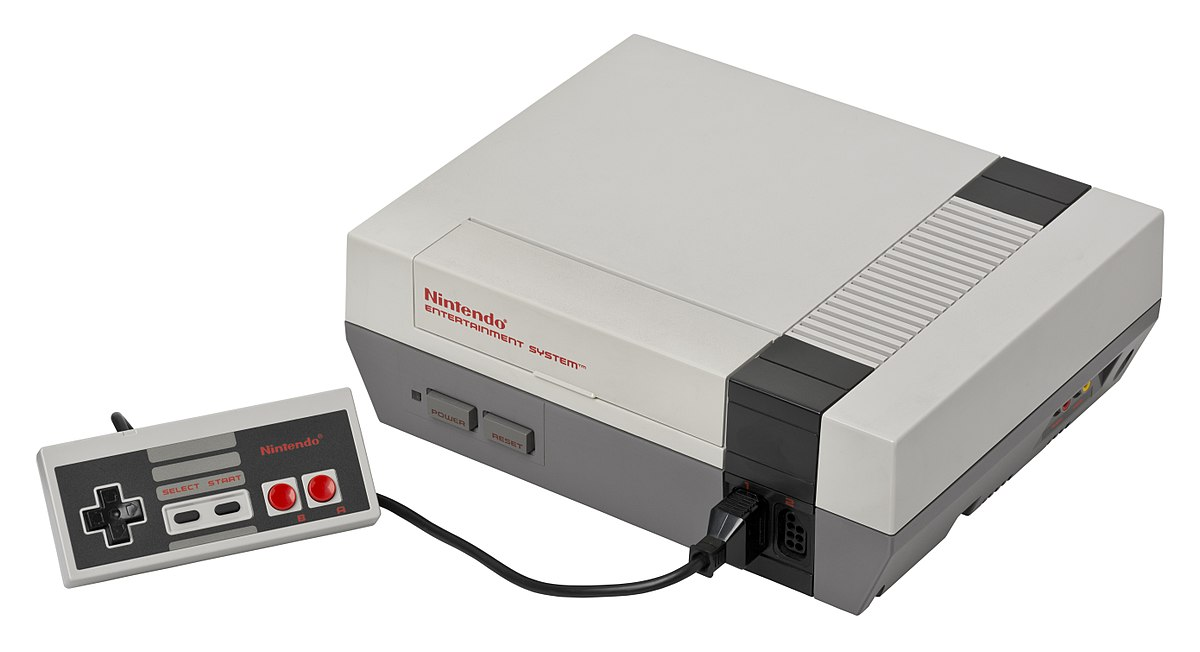
\includegraphics[width=\textwidth]{nes}
			
			
\includegraphics[width=\textwidth]{supermario}
		\end{column}
		\begin{column}{0.64\textwidth}
			\begin{itemize}
				\pause\item Released in \textbf{1983}
				\pause\item Sold as the \textbf{Famicom} (Family Computer) in Japan
				\pause\item Nearly \textbf{62 million} units sold worldwide
				\pause\item Biggest selling game: \textbf{Super Mario Bros}
				\pause\item Credited with reviving the games industry after the \textbf{video game crash} of the early 80s
			\end{itemize}
		\end{column}
	\end{columns}
\end{frame}

\begin{frame}{Nintendo Entertainment System (NES)}
	\begin{columns}
		\begin{column}{0.32\textwidth}
			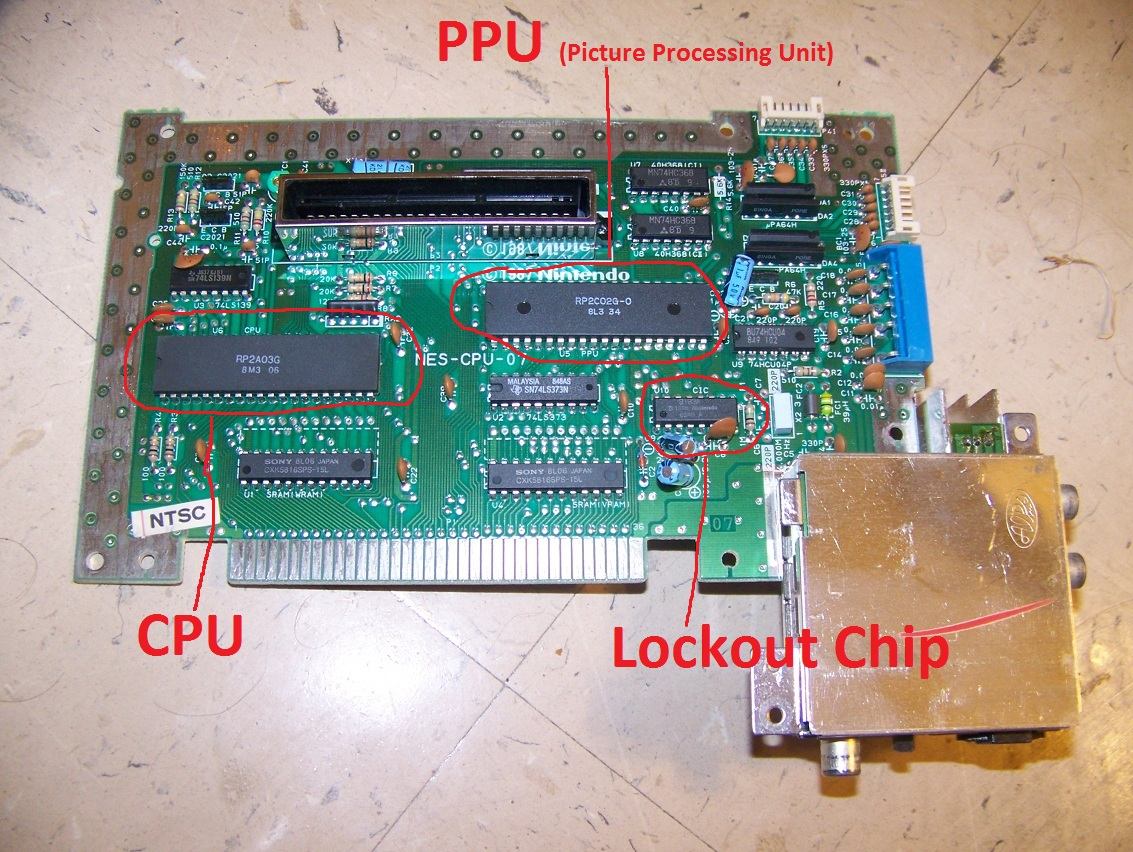
\includegraphics[width=\textwidth]{nes_motherboard}
		\end{column}
		\begin{column}{0.64\textwidth}
			\begin{itemize}
				\pause\item CPU: Ricoh 2A03 (closely based on MOS 6502)
				\pause\item Picture Processing Unit (PPU): Ricoh RP2C02 or RP2C07
				\pause\item RAM: 2 kilobytes for CPU + 2 kilobytes for PPU
				\pause\item Cartridge ROM: up to 1 megabyte, but typically less
				\pause\item Screen resolution: 256 $\times$ 240
			\end{itemize}
		\end{column}
	\end{columns}
\end{frame}

\begin{frame}{Technical limitations}
	\begin{itemize}
		\pause\item Around \textbf{2270 CPU cycles per frame}
		\pause\item Only \textbf{2 kilobytes} of writable memory to work with
		\pause\item 6502 instruction set is limited
			\begin{itemize}
				\pause\item 8-bit integer maths only
			\end{itemize}
		\pause\item The following are possible but need implementing as subroutines:
			\begin{itemize}
				\pause\item $>8$ bit numbers
				\pause\item Multiplication
				\pause\item Division
				\pause\item Fractional numbers
			\end{itemize}
	\end{itemize}
\end{frame}

\begin{frame}{Graphical limitations}
	\begin{itemize}
		\pause\item Display is made up of \textbf{sprites} and \textbf{background}
		\pause\item Sprites:
			\begin{itemize}
				\pause\item Maximum 64 on screen
				\pause\item Maximum 8 on the same scanline (horizontal line)
				\pause\item $8 \times 8$ pixels, 3 colours + transparency
				\pause\item Can flip horizontally or vertically
				\pause\item No rotation, scaling etc.
			\end{itemize}
		\pause\item Background:
			\begin{itemize}
				\pause\item Made of $8 \times 8$ pixel tiles
				\pause\item $32 \times 32$ blocks must share the same 4-colour palette
				\pause\item Limitations on types of scrolling
			\end{itemize}
	\end{itemize}
\end{frame}

\begin{frame}
	\begin{center}
		\url{https://wiki.nesdev.com/w/index.php/Limitations}
	\end{center}
\end{frame}

\begin{frame}{Examples of NES games}
	\begin{center}
		\url{https://youtu.be/um-GMygsRg4}
	\end{center}
\end{frame}

\part{Developing for the NES}
\frame{\partpage}

\begin{frame}{Tools}
	\begin{itemize}
		\pause\item An \textbf{emulator}
			\begin{itemize}
				\pause\item Recommended: FCEUX
				\item \url{http://www.fceux.com/}
			\end{itemize}
		\pause\item An \textbf{assembler}
			\begin{itemize}
				\pause\item Recommended: NESASM
				\item {\footnotesize\url{https://github.com/edpowley/nesasm/releases}}
			\end{itemize}
		\pause\item A \textbf{sprite editor}
			\begin{itemize}
				\pause\item Recommended: YY-CHR
				\item \url{https://www.romhacking.net/utilities/119/}
			\end{itemize}
		\pause\item A \textbf{text editor}
	\end{itemize}
\end{frame}

\begin{frame}{Live coding videos}
	\begin{itemize}
		\pause\item \url{bit.ly/comp310}
		\pause\item I expect you to work through these \textbf{in your own time}
		\pause\item Timetabled workshops are mostly for \textbf{working on your projects} and getting \textbf{support}
		    (although there will also be a bit of taught material)
	\end{itemize}
\end{frame}

\begin{frame}{Let's jump in!}
	\begin{itemize}
		\pause\item \url{http://nintendoage.com/forum/messageview.cfm?catid=22&threadid=7974}
		\pause\item Download \texttt{controller.zip}
	\end{itemize}
\end{frame}

\begin{frame}{Exercise}
	Modify \texttt{controller.asm} so that all of Mario moves left and right, not just the back of his head...
\end{frame}



\end{document}
